\documentclass[../Thesis.tex]{subfiles}
\graphicspath{{\subfix{../figures/}}}
% \epstopdfsetup{outdir={../figures/}}
\usepackage{xr}
\externaldocument{C4 Method}
\externaldocument{../_BackMatter/Appendix1}
\begin{document}

\chapter{Results}
\textcolor{red}{en intro til hvad der kommer til at være resultater ift. }

In this section, we will investigate how the algorithms \autoref{alg:Gobs1} and \autoref{alg:ND} works in junction and individually. We shall observe how the algorithms can fail and what may be done to correct such cases.

\textcolor{red}{Overordnet pointe er at genere forskellige mulige graphisce modeller, som senere ville kunne bruges til at lave PGM el.l. Er nok bedst som et ekspolartivt værktøj, og vi undersøger her forskellige situationer, og hvornår der kan ske fejl ud fra om det er lange kæder af kausalitet eller mere komplekse strukturer}

% Initially, a few simple examples involving exponentiated multivariate Gaussians $\boldsymbol Y $.


\newpage
\section{Gaussian chains}
In this section we discuss the errors made from the assumption that indirect effects can be computed as a sum of powers of the direct effects, i.e. $G_{indir} = \sum_{k\geq 1} G_{dir}^k$. In particular, on a theoretical level, we shall observe the error in $G_{obs}$ based on the above assumption of how similarities are \textit{convolved} which we equate with the noise $N$ from \autoref{subseq:Robustness to noise}, although it is a systematic error. To do this, we shall in this section use a multivariate Gaussian to be able to control the correlation and as an extension of this, the mutual information between pairs of random variables. As we already know, correlation and mutual information is independent of the mean and variance of each of the variables however for a bivariate Gaussian the mutual information is given by the correlation as stated in the following proposition.
\begin{proposition}\label{prop:MI bivariate gaussian}
    Given a bivariate normal distribution $\boldsymbol X \sim \mathcal{N}\left(\boldsymbol \mu,  \Sigma\right)$ where
    $$\Sigma =
        \begin{bmatrix}
            \sigma_1^2             & \rho \sigma_1 \sigma^2 \\
            \rho \sigma_1 \sigma_2 & \sigma_2^2
        \end{bmatrix}
    $$
    Then the mutual information $I\left(X_1, X_2\right) = -\frac{1}{2}\ln \left(1 - \rho^2\right)$.
\end{proposition}
\begin{proof}
    This follows by direct computation Using e.g. that $I(X_1, X_2) = h(X_1) + h(X_2) - h(X_1, X_2)$
\end{proof}
Thus, if we know a correlation structure of a Gaussian random vector, we also know the mutual information between every pair of variables which we shall now use in the following made up example. Namely, what we shall denote as a Gaussian chain defined as a Gaussian random vector in the following way. Let $\boldsymbol X$ be a $d$-dimensional Gaussian random vector, the $\boldsymbol X$ is a standard Gaussian chain if it can be written in the following way in terms of $d$ independent standard normal variables $Z_i$ up to a permutation i.e. there exists a permutation of the variables of the random vector $\boldsymbol X$ that permits the following structure.
\begin{equation}\label{eq:Gaussian chain def}
    \begin{split}
        X_1 & = Z_1                                                      \\
        X_2 & = \rho_{1,2} X_1 + \sqrt{1 - \rho_{1,2}^2} Z_2             \\
        X_3 & = \rho_{2,3} X_2 + \sqrt{1 - \rho_{2,3}^2} Z_3             \\
            & \vdots                                                     \\
        X_d & = \rho_{d-1, d} X_{d-1} + \sqrt{1 - \rho_{d-1, d}^2} Z_{d}
    \end{split}
\end{equation}
It follows that the marginals have variance $1$ as clearly $\text{Var} \left[X_1\right] = \text{Var}\left[Z_1\right] = 1$ and for $i > 1$, $\text{Var}\left[X_i\right] = \rho_{i-1,i}^2 \text{Var}\left[X_{i-1}\right] + \left(1 - \rho_{i-1,i}^2\right) \text{Var} \left[Z_i\right] = 1$ by independence of $X_{i-1}$ and $Z_i$. Thus, the above structure also implies the Cholesky factorization of the correlation matrix for $\boldsymbol X$, namely
$$L = \begin{bmatrix}
        1                          &                                   &                                                        &        &                          \\
        \rho_{1,2}                 & \sqrt{1 - \rho_{1,2}^2}           &                                                        &        &                          \\
        \rho_{2,3}\rho_{1,2}       & \rho_{2,3}\sqrt{1 - \rho_{1,2}^2} & \sqrt{1 - \rho_{2,3}^2}                                &        &                          \\
        \vdots                     &                                   &                                                        & \ddots &                          \\
        \prod_{i=2}^d \rho_{i-1,i} & \dots                             & \sqrt{1 - \rho_{j-1,j}^2} \prod_{i=j+1}^d \rho_{i-1,i} & \dots  & \sqrt{1- \rho_{d-1,d}^2}
    \end{bmatrix}$$
Which will allow us to both sample from such a chain and calculate $G_{dir}$ and $G_{obs}$ theoretically. However, in this example, it is easier to calculate the correlation between the variable $X_i$ and $X_j$ directly. As the variance of each variable is $1$ we simply calculate the covariance. We assume without loss of generality that $i < j$ whence
$$\text{Cov}\left[X_i, X_j\right] = \text{Cov}\left[X_i, \rho_{j-1,j} X_{j-1} + \sqrt{1 - \rho_{j-1,j}^2}Z_j\right] = \rho_{j-1,j} \text{Cov}\left[X_i, X_{j-1}\right]$$
which by induction implies $\rho_{i,j} = \prod_{k=i+1}^{j} \rho_{k-1,k} = \rho_{j,i}$. At this point, we are almost ready to use the algorithms from the previous chapter. First, we will only use \autoref{alg:ND} to deconvolve the network based on theoretical correlations and later mutual information. However, before doing so, we note that from the definition in \autoref{eq:Gaussian chain def} the random variable $\boldsymbol X$ exhibits a Markovian property. Namely, the $X_i$ above can be understood discrete stochastic process as they are successively drawn based only on the previous variable $X_{i-1}$ i.e. $f\left(X_i \mid X_{i-1}, X_{i-1} , \dots , X_{1}\right) = f\left(X_i \mid X_{i-1}\right)$. Thus, if the algorithm works as intended, we should observe that the deconvolved network is a \textit{chain} of variables as shown in the \autoref{fig:gaussian chain expected res}
\begin{figure}[h]
    \centering
    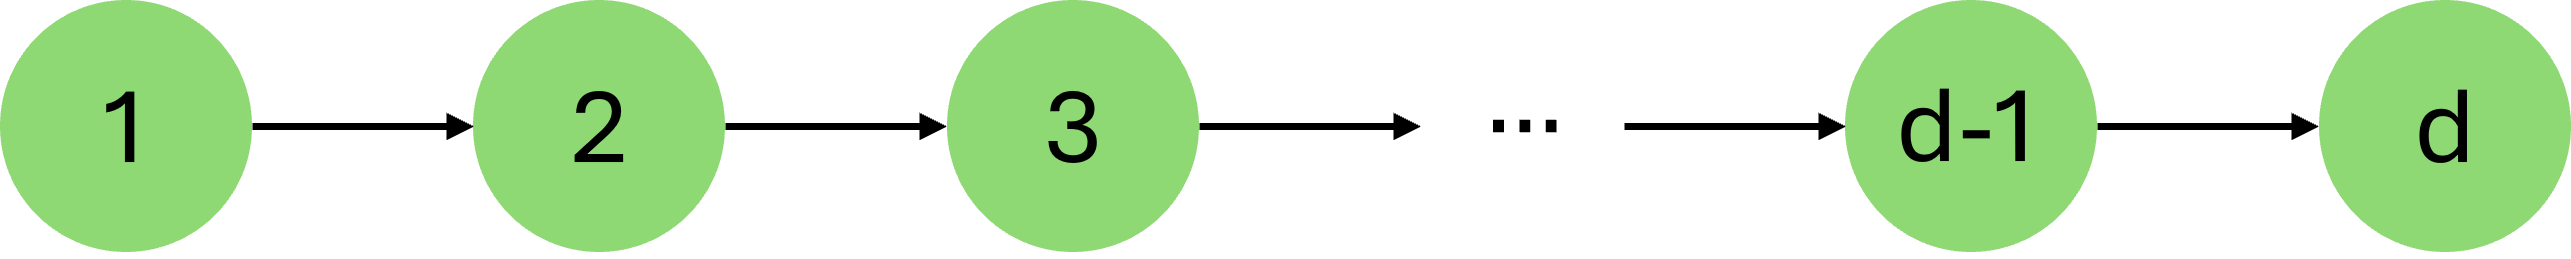
\includegraphics[width = .7\linewidth]{figures/ND examples/Gaussian chain.png}
    \caption{The graphical representation of a Gaussian chain. Arrows signify a possible causal structure. If furthermore, one assumes that $X_1$ is generated first, then $X_2$ and so on, this is the only causal structure that would make sense.}
    \label{fig:gaussian chain expected res}
\end{figure}
Thus, we now have the expected result, and we proceed with using correlation and mutual information to try and rediscover this structure in the following two sections

\subsection{Gaussian chain deconvolution using correlation}
In this section, we will use the observed correlation i.e. $\rho_{i,j} = \prod_{k=i+1}^{j} \rho_{k-1,k}$ for the elements of $G_{obs}$ with $i< j$. Note that although it makes sense to consider the correlation between a variable and itself, we shall as discussed before set the diagonal to $0$. Furthermore, we have the choice of using either a symmetrical $G_{obs}$ or a (upper or lower) triangular $G_{obs}$. We shall first use an upper triangular $G_{obs}$ but before using deconvolving using \autoref{eq:Gdir from Gobs} we note that we can actually get the result theoretically. Also, as $G_{obs}$ is in this case strictly upper triangular, the spectral radius is $0$ and hence we have no problems with converge of the infinite sum of powers of (the uniquely defined) $G_{dir}$. From the above, it is clear that $G_{obs}$ is given as follows
\begin{equation}\label{eq:Gaussian chain G_obs trinagular form}
    G_{obs} = \begin{bmatrix}
        0 & \rho_{1,2} & \rho_{1,2}\,\rho_{2,3} & \dots & \prod_{k=2}^{d} \rho_{k-1,k} \\
          & 0          & \rho_{2,3}             & \dots & \prod_{k=3}^{d} \rho_{k-1,k} \\
          &            & \ddots                 &       & \vdots                       \\
          &            &                        & 0     & \rho_{d-1,d}                 \\
          &            &                        &       & 0
    \end{bmatrix}
\end{equation}
Now, let $G_{dir}$ be given as follows
$$G_{dir} = \begin{bmatrix}
        0 & \rho_{1,2} &            &        &              \\
          & 0          & \rho_{2,3} &        &              \\
          &            & \ddots     & \ddots &              \\
          &            &            & 0      & \rho_{d-1,d} \\
          &            &            &        & 0
    \end{bmatrix}$$
then $G_{dir}^2$ is given by
$$G_{dir}^2 = \begin{bmatrix}
        0 & 0 & \rho_{1,2}   \, \rho_{2,3} &                          &        &                               \\
          & 0 & 0                          & \rho_{2,3} \, \rho_{3,4} &        &                               \\
          &   & \ddots                     & \ddots                   & \ddots &                               \\
          &   &                            & 0                        & 0      & \rho_{d-2,d-1}\, \rho_{d-1,d} \\
          &   &                            &                          & 0      & 0
    \end{bmatrix}$$
It is not hard to show that in fact $\sum_{k\geq} G_{dir}^k = \sum_{k=1}^d G_{dir}^k = G_{obs}$. Thus, if we know a graph topological ordering of the variables corresponding to the structural causal model, we completely recover (without any error) the direct dependencies/correlation from to the initial definition in \autoref{eq:Gaussian chain def}. This actually holds for a general \textit{chain} where $Z_i$ can follow any distribution as long as they are independent as the above computations did not use the fact that $Z_i$ follows a standard Gaussian. From this, we might think that if we have a topological ordering of the variables this is the preferred method, and it is as long as correlation is a good enough measure of similarity/codependency. Albeit this is only shown for the special case of a chain, in \autoref{sec:General Gaussian graph} we consider the more general case and conclude that this indeed holds. Regarding the comment on correlation being a good enough measure of similarity, a prototypical case is when joint probability density function of two variables resemble a parabola. Namely, let $X_1\sim \mathcal{U}\left(0,1\right)$ and $X_2 \mid X_1 \sim \mathcal{N}\left(1 - 4\left(x_1 - 1/2\right)^2 , \sigma^2\right)$ i.e. the joint distribution function is a parabola with a Gaussian noise added along the second dimension. In \autoref{fig:MI parabola example}, $1000$ samples from this distribution is shown for $\sigma = 1/10$ along with the expectation $\mathbb{E}\left[X_2 | X_1\right]$. It is not hard to show that the covariance between $X_1$ and $X_2$ is $0$ however we clearly see a relationship between the two variables. In fact, computing the mutual information results in $I\left(X_1,X_2\right) \approx 1.030$ implying $X_1 \not\perp X_2$ i.e. there exists a higher order (non-linear) dependency. Thus, if the algorithm permits, we would prefer mutual information to correlation as we can then use observed higher order relationships to infer a causal structure.
\begin{figure}[h]
    \centering
    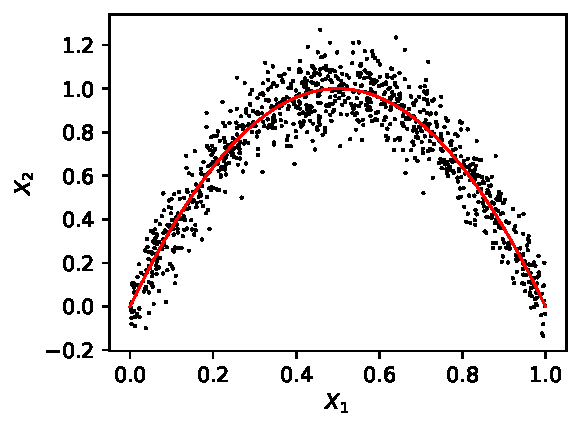
\includegraphics[width=.55\linewidth]{figures/Mutual information figures/parabola example.pdf}
    \caption{1000 samples generated from $X_1\sim \mathcal{U}\left(0,1\right)$ and $X_2 \mid X_1 \sim \mathcal{N}\left(1 - 4\left(x_1 - 1/2\right)^2 , \sigma^2\right)$ with $\sigma = 1/10$. The mutual information is calculated theoretically to be $I\left(X_1,X_2\right) \approx 1.030$ and repeated simulations show that the empirical correlation is symmetric around $0$ supporting the claim that the underlying correlation is in fact $0$} % 1.0296516475133333
    \label{fig:MI parabola example}
\end{figure}
On a more technical point of view, we note that mutual information is a measure of how dense the joint distribution is, invariant to scale. In a way, it is a measure of how close the joint distribution is to a lower dimensional manifold.

We proceed with a $10$-Gaussian chain defined by the following correlations:
\begin{equation}\label{eq:Example Gaussian chain}
    \begin{aligned}
        \rho_{1,2} & = 0.6, & \rho_{2,3} & = 0.5, & \rho_{3,4}  & = 0.4 \\
        \rho_{4,5} & = 0.2, & \rho_{5,6} & = 0.9, & \rho_{6,7}  & = 0.8 \\
        \rho_{7,8} & = 0.9, & \rho_{8,9} & = 0.8, & \rho_{9,10} & = 0.7
    \end{aligned}
\end{equation}
We have chosen correlations of different sizes to check if the deconvolution is robust in presence of both strong and weak links. In particular, $X_5$ is only $\rho_{4,5}^2 = 4\%$ of $X_4$ and the remaining $96\%$ is noise/indescribable variance i.e. a very weak link between the first part of the chain up to and including $X_4$ and the rest. However, as discussed above, if let $G_{obs}$ be upper triangular, we should completely rediscover these direct relations which is indeed also the case. In particular, from \autoref{fig:Gaussian chain triangular G_obs using correlation} we observe that the inferred network, represented by $G_{dir}$, is indeed a chain of variables and is exactly equal to the theoretical $G_{dir}$ as we would expect (up to very small rounding errors of the size $10^{-16}$). The \textit{estimated} $G_{dir}$ is also shown as a directed graph which the initial topological assumption implies, with edges wherever $G_{dir}$ is non-zero.
\begin{figure}[h]
    \centering
    \begin{subfigure}[t]{0.49\textwidth}
        \centering
        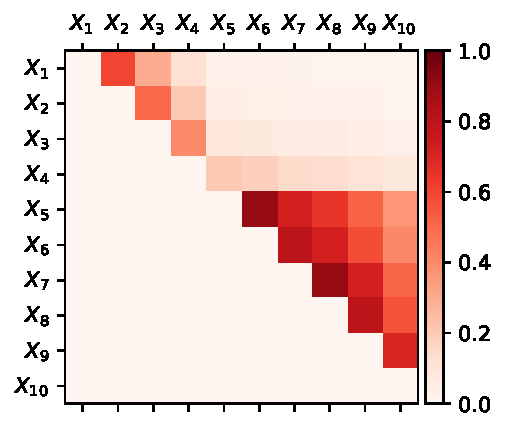
\includegraphics[width=.95\linewidth]{figures/Gaussian Chain Theoretical/triangular G obs.pdf}
        \caption{$G_{obs}$}
        % \label{fig:Gaussian 3x3 large s}
    \end{subfigure}
    \hfill
    \begin{subfigure}[t]{0.49\textwidth}
        \centering
        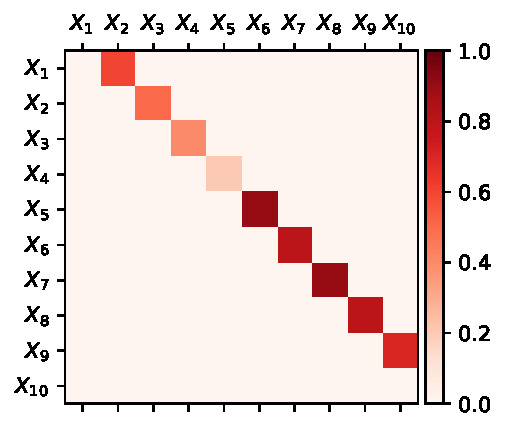
\includegraphics[width=.95\linewidth]{figures/Gaussian Chain Theoretical/G dir from triangular G obs.pdf}
        \caption{$G_{dir}$}
        \label{subfig:Gaussian chain triangular G_obs using correlation - G_dir}
    \end{subfigure}
    \\[\baselineskip]
    \begin{subfigure}[t]{0.49\textwidth}
        \centering
        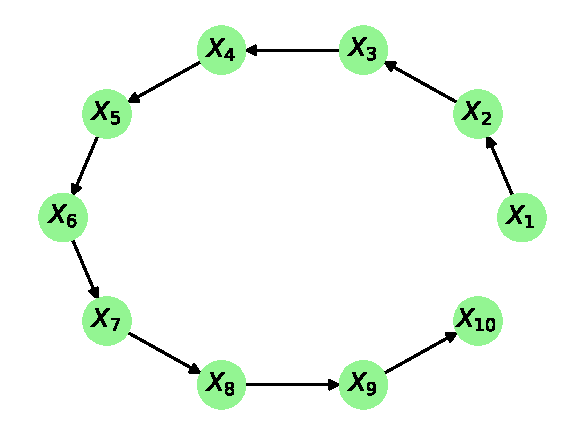
\includegraphics[width=.9\linewidth]{figures/Gaussian Chain Theoretical/Chain graph from triangular G obs.pdf}
        \caption{$G_{dir}$ as a digraph}
        % \label{fig:Gaussian 3x3 large s}
    \end{subfigure}
    \caption{Results from using an upper triangular $G_{obs}$ and correlation to infer the causal network structure. (a) shows the upper triangular $G_{obs}$ with the correlation between every pair of variables. (b) shows the deconvolved $G_{obs}$ and as we expect, the superdiagonal contains the original correlations given in \autoref{eq:Example Gaussian chain}. (c) shows $G_{dir}$ represented as a digraph and matches the expected result.}
    \label{fig:Gaussian chain triangular G_obs using correlation}
\end{figure}
We now proceed to investigate what happens when we remove the prior information of the topological ordering. Namely, if $G_{obs}$ is no longer triangular but symmetric. In particular, let $T_{dir}$ be given as $G_{dir}$ above. We then have that $G_{dir}$ in the symmetric case is $T_{dir} + T_{dir}^T$ and similarly for $G_{obs}$, $G_{obs} = T_{obs} + T_{obs}^T$. Clearly, $I + G_{obs}$ is positive definite as it is a proper correlation matrix. However, that also implies that we might have eigenvalues of $G_{obs}$ less than or equal to $-1/2$ which we know from \autoref{subsec:Setup and assumptions} is not the result of a $G_{dir}$ such that \autoref{eq:Gobs from Gdir} holds as then the infinite sum diverges. However, as $-1$ is not an eigenvalue of $G_{obs}$, we will investigate what happens if one tries to use \autoref{eq:Gdir from Gobs} anyway.

First, we shall however discuss the errors being made using the symmetric $G_{obs}$ and $G_{dir}$. Namely, we investigate the powers of $G_{dir}$:
$$G_{dir}^2 = \left(T_{dir} + T_{dir}^T\right)^2 = T_{dir}^2 + \left(T_{dir}^T\right)^2 + T_{dir} T_{dir}^T + T_{dir}^T T_{dir}$$
Higher power can be calculated similarly, but for the second power we already observe an error. The first two terms corresponds to a reflection of the second order effects that we saw above and know to be true, whence the final two terms, that add to a diagonal matrix, is an error and will propagate with higher order powers of $G_{dir}$. Through simple calculation the resulting error is
$$T_{dir} T_{dir}^T + T_{dir}^T T_{dir} = \begin{bmatrix}
        \rho_{1,2}^2 + \rho_{2,3}^2 &                             &        & \\
                                    & \rho_{2,3}^2 + \rho_{3,4}^2 &        & \\
                                    &                             & \ddots & \\
                                    &   &   & \rho_{d-2,d-1}^2 + \rho_{d-1,d}^2
    \end{bmatrix}$$
Thus, for chains, we expect larger errors for sub-chains with strong links i.e. a subgraph of a chain that is also a chain where the correlation from one variable to the next is large. Using $G_{obs} = T_{obs} + T_{obs}^T$ we have that the smallest eigenvalue is approximately $\lambda_{\min} \approx -0.92263$ thus, multiplying $G_{obs}$ with a constant $c_s < 0.54192$ will make $G_{dir}$ have spectral radius at most $1$. The results vary with one or two edges for the choice of $c_s$ and in the following we have chosen $c_s = 0.53651$ resulting in $\rho\left(G_{dir}\right) \approx 0.98020$ and $\tilde{G}_{obs}$ and $\tilde{G}_{dir}$ as seen in \autoref{fig:Gaussian chain symmetric G_obs using correlation}. From \autoref{subfig:Gaussian chain symmetric G_obs using correlation - G_dir} we see that some correlation/association seem to bleed to variables $2$ or $3$ edges away which we of course know is not true given the Markov property discussed above. However, it is also clear that the error here is that the original assumption does not hold since using a symmetric $G_{obs}$ imply that the measure of similarity flows both ways where in this case it is very much unidirectional.

From \autoref{fig:Gaussian chain symmetric G_obs using correlation} conclude that we are somewhat able to rediscover the causal structure. Not surprisingly, we observe that the weak link between $X_4$ and $X_5$ is one of the first to break and that we observe some extra edges between the later more strongly linked sub-chain as by the above discussion. Finally, before presenting the results for the unscaled $G_{obs}$ (such that the smallest eigenvalue is larger than $-1/2$) we note that changing the parameter $\alpha$ in \autoref{alg:ND} did not have much of an effect indicating that the network is quite sparse (as we also know it to be) as even removing $65\%$ of the smallest correlations from $G_{obs}$ did not have any effect. The chosen threshold of $t=0.2$ on $G_{dir}$ seemed to be the best compromise of a connected graph and the density of the edges (although this is somewhat biased from prior knowledge of the true graphical structure).
% Also, trying to have $1$ in the diagonal instead of $0$ worsened the result
\begin{figure}[h]
    \centering
    \begin{subfigure}[t]{0.49\textwidth}
        \centering
        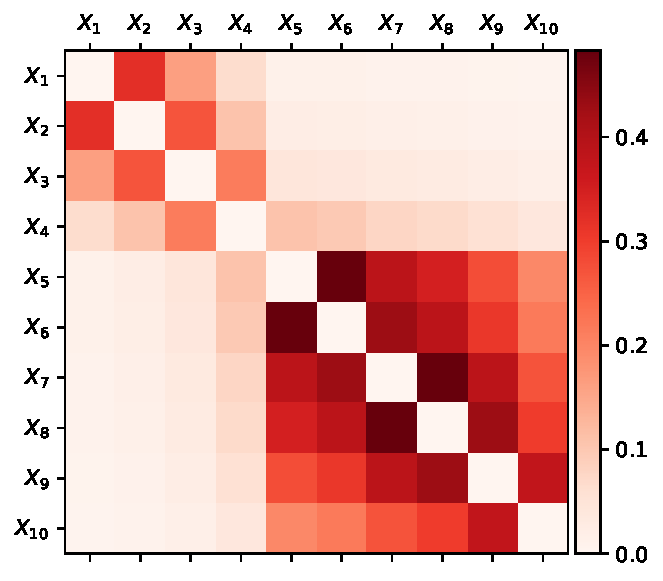
\includegraphics[width=.95\linewidth]{figures/Gaussian Chain Theoretical/symmetric G obs.pdf}
        \caption{$G_{obs}$}
        % \label{}
    \end{subfigure}
    \hfill
    \begin{subfigure}[t]{0.49\textwidth}
        \centering
        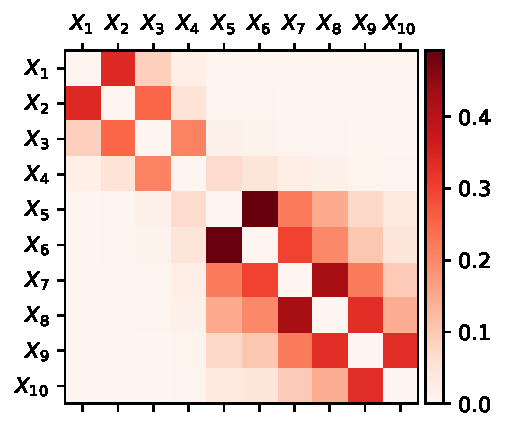
\includegraphics[width=.95\linewidth]{figures/Gaussian Chain Theoretical/G dir from symmetric G obs.pdf}
        \caption{$G_{dir}$}
        \label{subfig:Gaussian chain symmetric G_obs using correlation - G_dir}
    \end{subfigure}
    \\[\baselineskip]
    \begin{subfigure}[t]{0.49\textwidth}
        \centering
        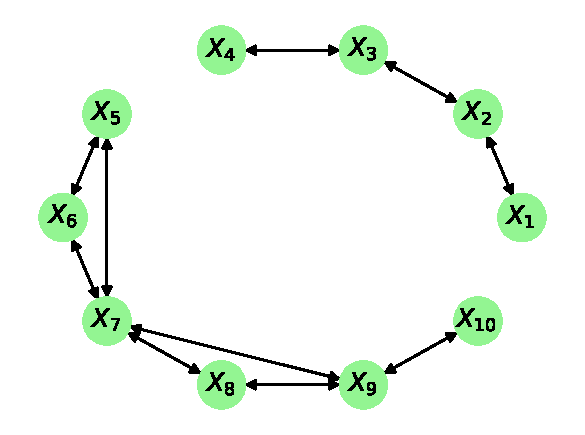
\includegraphics[width=.9\linewidth]{figures/Gaussian Chain Theoretical/Chain graph from symmetric G obs.pdf}
        \caption{$G_{dir}$ as a graph}
        % \label{}
    \end{subfigure}
    \caption{Using a symmetric $G_{obs}$ as shown in (a), we observe that higher order effects start to emerge as can be seen in (b). The main response is still in the superdiagonal and subdiagonal as we expect, where some similarity seems to bleed to nearby nodes/variables thus making the threshold used important for the resulting graph. For (c), a threshold $t=0.2$ was used to obtain a decent compromise between connectedness and denseness of the direct association.}
    \label{fig:Gaussian chain symmetric G_obs using correlation}
\end{figure}
% minimize error in g_dir from equation on error?
Finally, we try using the unscaled $G_{obs}$ in \autoref{eq:Gdir from Gobs}. Interestingly, we find that the true structure emerges as can be seen from \autoref{fig:Gaussian chain symmetric G_obs using correlation - unscaled}. Although the \textit{correlations} in \autoref{subfig:Gaussian chain symmetric G_obs using correlation - G_dir - unscaled} are not really correlations they do resemble those discovered in \autoref{subfig:Gaussian chain triangular G_obs using correlation - G_dir}. On closer inspection, it is not apparent how they are related except that it is a non-linear relationship. Although in this case it seemed to work not rescaling $G_{obs}$ in order to discover the causal structure we will in general not apply this to real world scenarios as the method is not well-defined in terms of assumptions and what the resulting $G_{dir}$ should be interpreted as.
\begin{figure}[h]
    \centering
    \begin{subfigure}[t]{0.49\textwidth}
        \centering
        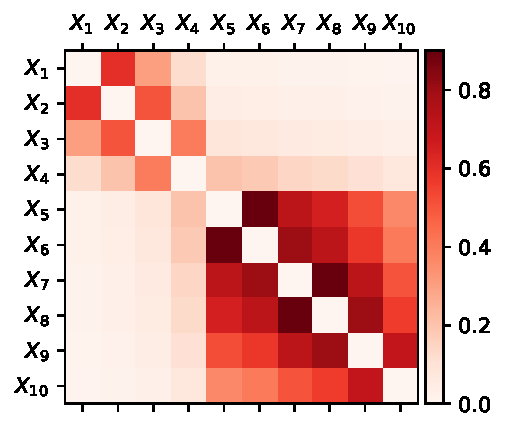
\includegraphics[width=.95\linewidth]{figures/Gaussian Chain Theoretical/symmetric G obs - unscaled.pdf}
        \caption{$G_{obs}$}
        % \label{}
    \end{subfigure}
    \hfill
    \begin{subfigure}[t]{0.49\textwidth}
        \centering
        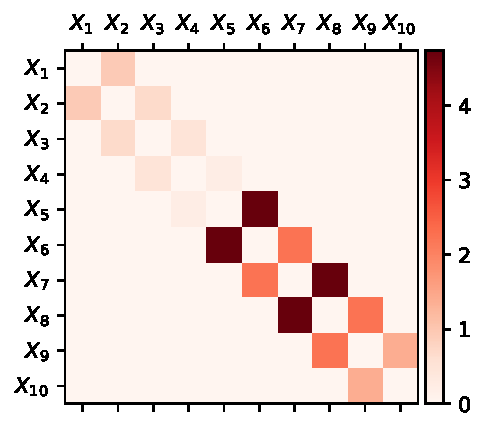
\includegraphics[width=.95\linewidth]{figures/Gaussian Chain Theoretical/G dir from symmetric G obs - unscaled.pdf}
        \caption{$G_{dir}$}
        \label{subfig:Gaussian chain symmetric G_obs using correlation - G_dir - unscaled}
    \end{subfigure}
    \\[\baselineskip]
    \begin{subfigure}[t]{0.49\textwidth}
        \centering
        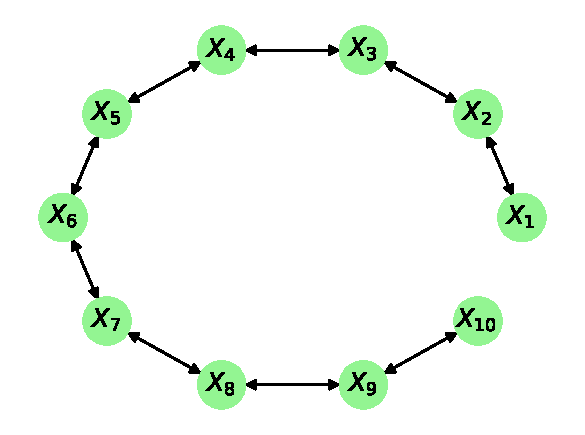
\includegraphics[width=.9\linewidth]{figures/Gaussian Chain Theoretical/Chain graph from symmetric G obs - unscaled.pdf}
        \caption{$G_{dir}$ as a graph}
        % \label{}
    \end{subfigure}
    \caption{Using an unscaled (symmetric) $G_{obs}$ results in a good recovery of the causal structure as seen in (b) and (c). However, at this point it is not clear whether it holds only for chains and using correlation or if it is a more general phenomenon.}
    \label{fig:Gaussian chain symmetric G_obs using correlation - unscaled}
\end{figure}
Thus, at this point we have a rather good understanding of how the method works on Gaussian chains if one uses correlation as a measure of association. Furthermore, if one knows (a plausible) topological ordering of the variables, we are able to perfectly rediscover the network of direct dependencies. However, as noted above, correlation is not always a good measure of similarity. Thus, we proceed experimenting with mutual information on the same Gaussian chain.

% Hvis den forkerte topologiske struktur benyttes, kan det give underlige resultater? -> Umiddelbart ja, for man ville ikke finde de rho i den originale definition, og der vil opstå effekter af et sådan forkert valgt topologisk orden.




\newpage

% Fejl regning for symmetrisk case? -> har undladt, da det er lidt mere komplekst og er nemmere at kvatificere med direkte udregninger
\subsection{Gaussian chain deconvolution using mutual information}
In this section, we continue the example from the previous section but instead of using correlation as a measure of similarity, we will use mutual information. Immediately, we note that mutual information or Copula entropy does not propagate as assumed in \autoref{eq:Gobs from Gdir}. As an example, from \autoref{prop:MI bivariate gaussian}, we know that the mutual information in the case of a Gaussian chain between a variable $X_i$ and the next variable $X_{i+1}$ is $-1/2 \log\left(1 - \rho_{i,i+1}^2\right)$ and similarly, using \autoref{eq:Gaussian chain G_obs trinagular form}, we have that
$$I\left(X_i, X_{i+2}\right) = -\frac{1}{2} \log \left(1 - \rho_{i,i+1}^2 \rho_{i+1,i+2}^2\right)$$
Thus, if $G_{dir}$ is triangular, using \autoref{eq:Gobs from Gdir} we should observe the following at the $(i,i+2)$ entry of $G_{obs}$ instead
$$\frac{1}{4} \log\left(1 - \rho_{i,i+1}^2\right)\,\log\left(1 - \rho_{i+1,i+2}^2\right)$$
I.e. we make an error (which we could take to be the noise $N$ from \autoref{subseq:Robustness to noise}) for second order effects equal to
$$-\frac{1}{2} \log \left(1 - \rho_{i,i+1}^2 \rho_{i+1,i+2}^2\right) - \frac{1}{4} \log\left(1 - \rho_{i,i+1}^2\right)\,\log\left(1 - \rho_{i+1,i+2}^2\right)$$
In general, for a Gaussian chain, we have that
$$N_{i,j} = -\frac{1}{2} \log\left( 1 - \prod_{k=i+1}^{j} \rho_{k-1,k}^2\right) - \left(-\frac{1}{2}\right)^{j-i}\prod_{k=i+1}^{j} \log\left(1 - \rho_{k-1,k}^2\right)$$
As we will see in \autoref{fig:2 chain MI error} and \autoref{fig:3 and 4 chain MI error}, for Gaussian chains we can expect some of the same bleeding behavior as observed in \autoref{fig:Gaussian chain symmetric G_obs using correlation} where we did not use the topological ordering but based the deconvolution on correlation. In particular, from the figures below, we see that for $3$-chains, the error is in many cases close to $0$ and for most combinations of $\rho_{1,2}$ and $\rho_{2,3}$ less than $0.1$. Furthermore, we note that the errors are the largest when it is a strongly connected $3$-chain i.e. if both $\rho_{1,2}$ and $\rho_{2,3}$ are close to $1$ which again resemble the behavior seen in the case of a symmetrical $G_{obs}$ using correlation as the measure of association although in this case, the error does not propagate to the same extend which we shall also see shortly, when applying the deconvolution algorithm. Notice that as as only the absolute value of the correlation matters, we only show the error for $\rho_{1,2}, \rho_{2,3} \geq 0$.
\begin{figure}[h]
    \centering
    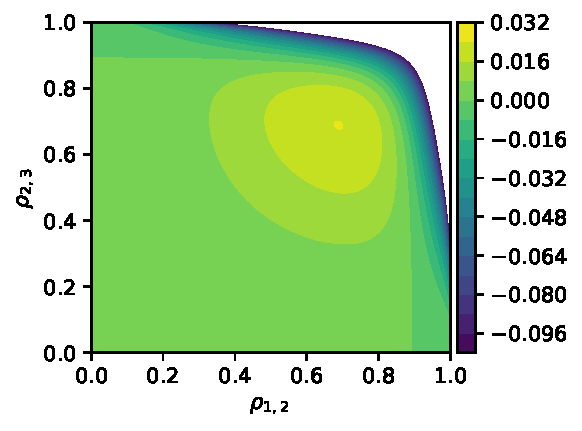
\includegraphics[width=.7\linewidth]{figures/Gaussian Chain Theoretical/2 chain error - MI.pdf}
    \caption{The error made by the assumption of $G_{obs}$ and $G_{dir}$ for second order observed effect. Although mutual information does not comply with the underlying assumptions, we observe that in the case of a Gaussian $2$-chain, we can expect the error to be relatively small.}
    \label{fig:2 chain MI error}
\end{figure}

We extend the above discussion to $4$- and $5$-chains (i.e. $j = i + 3$ and $j = i + 4$ in the above expression for $N_{ij}$) to see how the error propagates in more detail. This is shown in \autoref{fig:3 and 4 chain MI error} for three different scenarios of a $4$-chain and a single $5$-chain. In particular, as the error $N_{i,j}$ is symmetric in $\rho_{1,2}$, $\rho_{2,3}$ and $\rho_{3,4}$ (and $\rho_{4,5}$ in the case of a $5$-chain) and because it is hard to accurately show four or five dimensional surfaces, we keep to a fixed set of $\rho_{3,4}$ and $\rho_{4,5}$ when investigating. For the $4$-chain, choosing $\rho_{2,3} = 0.9$ (corresponding to mutual information about $0.8304$) approximately results in the same error as in \autoref{fig:2 chain MI error} and if $\rho_{2,3}$ is above e.g. $0.95$, we get a worse propagation of errors compared to the $3$-chain. Finally, from \autoref{subfig:Gaussian 5 chain MI error}, we see the same picture i.e. that keeping the correlations and hence information between subsequent variable low results in smaller errors in $G_{obs}$ and hence the inferred $G_{dir}$. Note that under the assumption of a topological ordering such that $G_{obs}$ is strictly upper triangular results in $\rho\left(G_{obs}\right) = 0$ such that no rescaling is necessary (although different choices of the base of the logarithm would have an effect on how much higher order associations influence $G_{dir}$).

% Ud fra plots, kan vi konkludere at fejlene ved at bruge den transformere G_obs ud fra correlation ikke er så lang væk fra det man ville få ud fra convolution af G_dir (under antagelse af at summen convergerer -> det gør den altid, fordi G_dir er strengt øvre trekant, så "inf" sum er faktisk begrænset/endelig)

Having obtained a good understanding of how shifting to mutual information instead of correlation in the case of Gaussian chains, we continue with the above example now using mutual information as the elements of $G_{obs}$ based on the correlation matrix from the previous section. Using a triangular $G_{obs}$ we observe similar behavior to that of original example using a triangular $G_{obs}$ but with correlation as can be seen from \autoref{fig:Gaussian chain triangular G_obs using mutual information}. In particular, we do not observe the same magnitude of bleeding effects as in \autoref{fig:Gaussian chain symmetric G_obs using correlation}. However, we observe
\begin{figure}[h]
    \centering
    \begin{subfigure}[t]{0.49\textwidth}
        \centering
        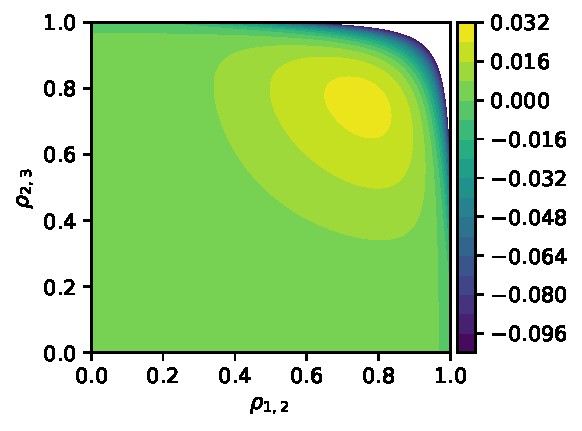
\includegraphics[width=.95\linewidth]{figures/Gaussian Chain Theoretical/3 chain error - MI - rho3 0_7.pdf}
        \caption{$4$-chain $\rho_{3,4} = 0.7$}
        % \label{fig:Gaussian 3x3 large s}
    \end{subfigure}
    \hfill
    \begin{subfigure}[t]{0.49\textwidth}
        \centering
        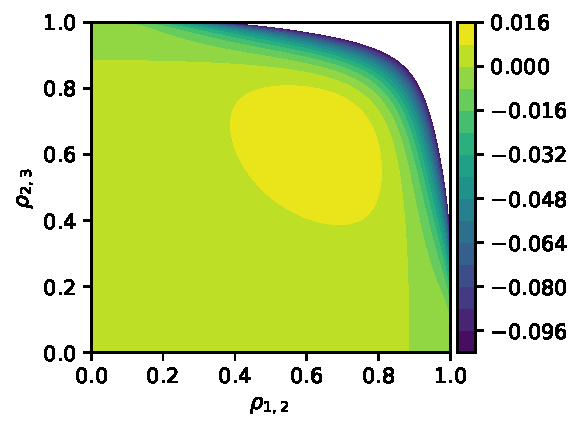
\includegraphics[width=.95\linewidth]{figures/Gaussian Chain Theoretical/3 chain error - MI - rho3 0_9.pdf}
        \caption{$4$-chain $\rho_{3,4} = 0.9$}
        % \label{fig:Gaussian 3x3 large s}
    \end{subfigure}
    \\[\baselineskip]
    \begin{subfigure}[t]{0.49\textwidth}
        \centering
        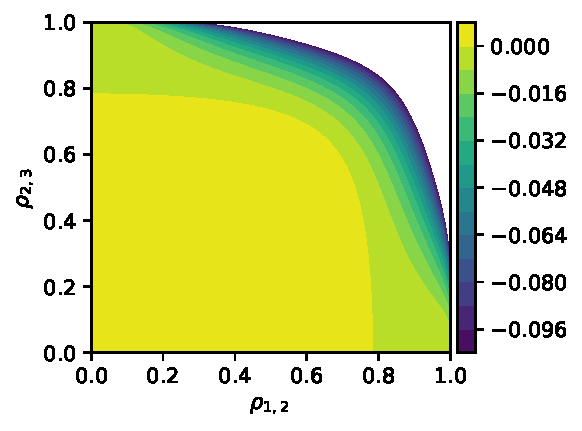
\includegraphics[width=.95\linewidth]{figures/Gaussian Chain Theoretical/3 chain error - MI - rho3 0_95.pdf}
        \caption{$4$-chain $\rho_{3,4} = 0.95$}
        % \label{fig:Gaussian 3x3 large s}
    \end{subfigure}
    \hfill
    \begin{subfigure}[t]{0.49\textwidth}
        \centering
        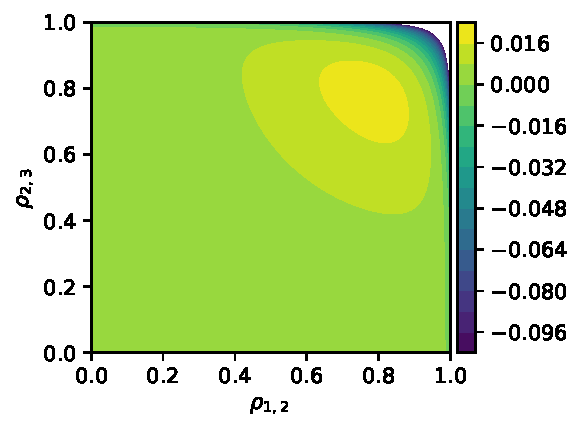
\includegraphics[width=.95\linewidth]{figures/Gaussian Chain Theoretical/4 chain error - MI - rho3 0_85 rho4 0_6.pdf}
        \caption{$5$-chain $\rho_{3,4} = 0.85$, $\rho_{4,5} = 0.6$}
        \label{subfig:Gaussian 5 chain MI error}
    \end{subfigure}
    \caption{Errors of convolving mutual information along a $4$-chain (a), (b), (c) and a $5$-chain (d). Due to symmetry in the expression of the error, only the first $2$ links i.e. $\rho_{1,2}$ and $\rho_{2,3}$ are varied on $[0,1]$ respectively. Only positive correlations are shown as the sign of the correlation cancels in the expression for the error. We note that large correlations and hence large mutual information on each edge results in larger error. In particular, when not too many of the links are strong, we have almost $0$ error.}
    \label{fig:3 and 4 chain MI error}
\end{figure}
the same tendency to miss weak connections as was also observed in \autoref{fig:Gaussian chain symmetric G_obs using correlation}. All in all, we get very good results using a triangular $G_{obs}$ even though mutual information does not have the same properties as correlation. In particular, this is what we expected as we have only used $\rho_{i,i+1} \leq 0.9$, from the above investigation of the error.
\begin{figure}[H]
    \centering
    \begin{subfigure}[t]{0.49\textwidth}
        \centering
        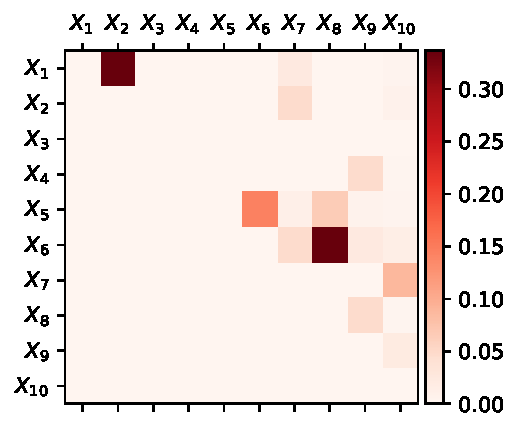
\includegraphics[width=.95\linewidth]{figures/Gaussian Chain Theoretical/triangular G obs - MI.pdf}
        \caption{$G_{obs}$}
        % \label{fig:Gaussian 3x3 large s}
    \end{subfigure}
    \hfill
    \begin{subfigure}[t]{0.49\textwidth}
        \centering
        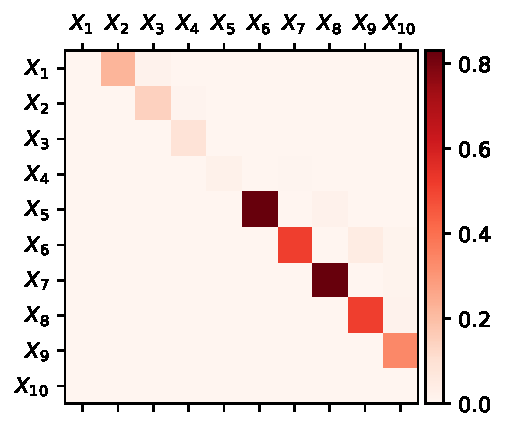
\includegraphics[width=.95\linewidth]{figures/Gaussian Chain Theoretical/G dir from triangular G obs - MI.pdf}
        \caption{$G_{dir}$}
        % \label{fig:Gaussian 3x3 large s}
    \end{subfigure}
    \\[\baselineskip]
    \begin{subfigure}[t]{0.49\textwidth}
        \centering
        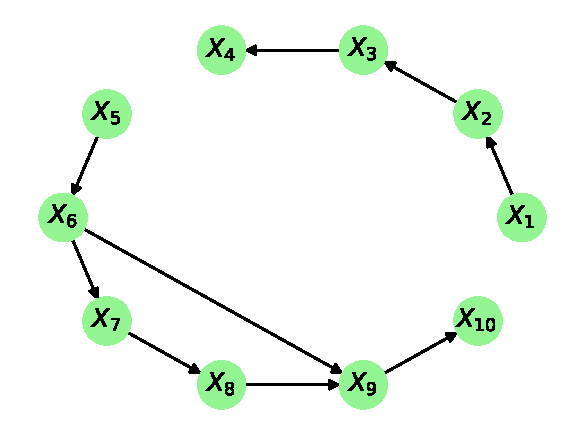
\includegraphics[width=.9\linewidth]{figures/Gaussian Chain Theoretical/Chain graph from triangular G obs - MI - cutoff 2_1e-2.pdf}
        \caption{$G_{dir}$ from $t = 2.1\cdot 10^{-2}$}
        % \label{fig:Gaussian 3x3 large s}
    \end{subfigure}
    \hfill
    \begin{subfigure}[t]{0.49\textwidth}
        \centering
        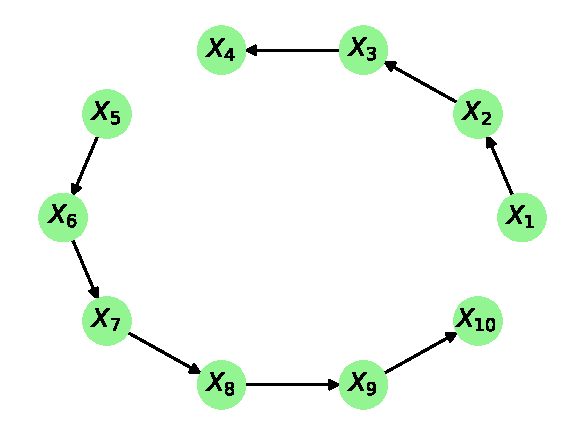
\includegraphics[width=.9\linewidth]{figures/Gaussian Chain Theoretical/Chain graph from triangular G obs - MI - cutoff 4_6e-2.pdf}
        \caption{$G_{dir}$ from $t = 4.6\cdot 10^{-2}$}
        % \label{fig:Gaussian 3x3 large s}
    \end{subfigure}
    \caption{Using mutual information as the measure of similarity as well as assuming a topological order i.e. making $G_{obs}$ strictly triangular as seen in (a) we almost perfectly infer $G_{dir}$ as seen in (b) except for $\left[G_{dir}\right]_{6,9}$. Choosing cutoffs $t = 2.1\cdot 10^{-2}$ (c) and $t = 4.6\cdot 10^{-2}$ (d) it is clear that adjusting the threshold we can get a better result than using a symmetric $G_{obs}$ with correlation.}
    \label{fig:Gaussian chain triangular G_obs using mutual information}
\end{figure}
Finally, we use the corresponding symmetric $G_{obs}$ (rescaled such that the largest absolute eigenvalue of $G_{dir}$ is $0.99$) which results in $G_{dir}$ and the graph using a threshold $t=4.88\cdot 10^{-2}$ shown in \autoref{fig:Gaussian chain symmetric G_obs using mutual information}. Again, we observe some bleeding on the more strongly connected sub-chain as with the symmetric $G_{obs}$ using correlation in \autoref{fig:Gaussian chain symmetric G_obs using correlation}. Again, we observe comparable results and note that increasing the threshold would disconnect $X_3$ and $X_4$ before removing the higher order effects.
\begin{figure}[h]
    \centering
    \begin{subfigure}[t]{0.49\textwidth}
        \centering
        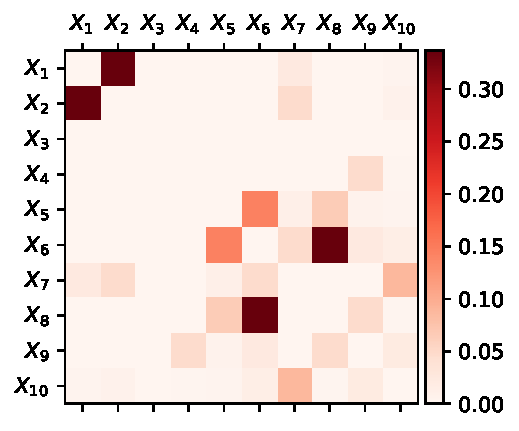
\includegraphics[width=.95\linewidth]{figures/Gaussian Chain Theoretical/symmetric G obs - MI.pdf}
        \caption{$G_{obs}$}
        % \label{fig:Gaussian 3x3 large s}
    \end{subfigure}
    \hfill
    \begin{subfigure}[t]{0.49\textwidth}
        \centering
        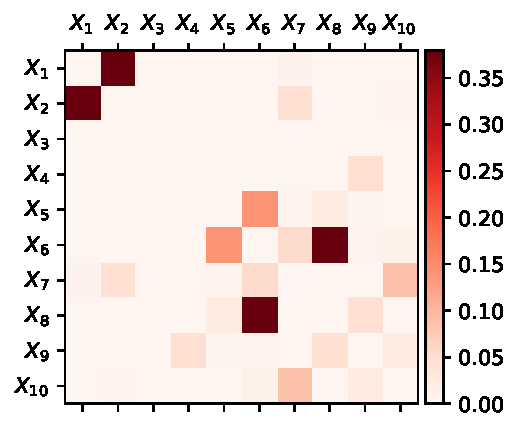
\includegraphics[width=.95\linewidth]{figures/Gaussian Chain Theoretical/G dir from symmetric G obs - MI.pdf}
        \caption{$G_{dir}$}
        % \label{fig:Gaussian 3x3 large s}
    \end{subfigure}
    \\[\baselineskip]
    \begin{subfigure}[t]{0.49\textwidth}
        \centering
        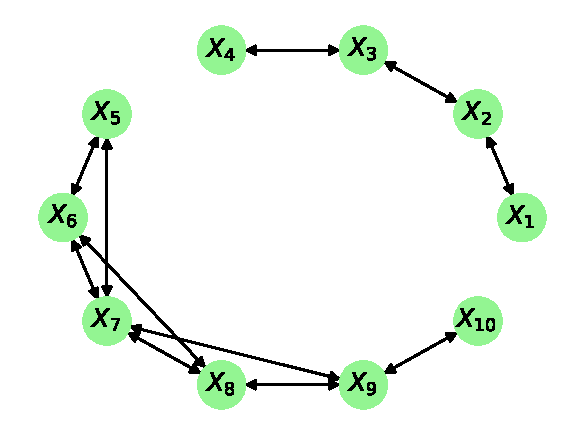
\includegraphics[width=.9\linewidth]{figures/Gaussian Chain Theoretical/Chain graph from symmetric G obs - MI - cutoff 4_88e-2.pdf}
        \caption{$G_{dir}$ as a graph}
        % \label{fig:Gaussian 3x3 large s}
    \end{subfigure}
    \caption{Using a symmetric $G_{obs}$ containing the observed mutual information (a) we infer a $G_{dir}$ (b) comparable to that if we had used correlation instead. Choosing the threshold $t = 4.88 \cdot 10^{-2}$ seem a good compromise between connectedness and density resulting in an almost identical discovered network structure to that of using a symmetric correlation $G_{obs}$.}
    \label{fig:Gaussian chain symmetric G_obs using mutual information}
\end{figure}

In conclusion, we have seen what errors can arise in the discovered network using both correlation and mutual information as the measure of association. Namely, long strongly connected chains seem to be a problem if one does not know a topological ordering of the variables, in which case these are heavily reduced  as seen in \autoref{fig:Gaussian chain triangular G_obs using correlation} and \autoref{fig:Gaussian chain triangular G_obs using mutual information}. Thus, we proceed in the next section by considering a more complicated underlying (Gaussian) network to observe if other unwanted effects can occur and if a topological ordering is necessary if the network is not simply a path.




\newpage
\section{Directed acyclic Gaussian graph}\label{sec:General Gaussian graph}
% where the Cholesky decomposed correlation matrix non-zero only in the diagonal and subdiagonal up to a permutation and possibly an operation with the transpose operator to ensure that 



% (with the superdiagonal and subdiagonal being equal of course) or if the correlation matrix is equivalent to such a matrix under a permutation matrix $P$ (a matrix of unit elements, summing to $1$ in every row and column) i.e. if $C$ is a Gaussian chain, so is $P^T C P$. An example of a $4$-Gaussian chain is
% $$C = \begin{bmatrix}
%     1 & \rho_{12} & 0 & 0\\
%     \rho_{21} & 1 & \rho_{23} & 0\\
%     0 & \rho{32} & 1 & \rho_{34}\\
%     0 & 0 & \rho_{43} & 1
% \end{bmatrix}$$




% \section{Examples}


\section{CE computation}\label{sec:gaussian MI error}
Gaussian example

\textcolor{red}{Example using Gaussian distribution and the error the algorithm makes.}


\begin{example} \label{ex:1}
    Exponentiated multivariate Gaussian

    Let us consider a simple case with $\mathbf{Y} = e^{\mathbf{X}}$ (element wise exponentiation) where $X \sim \mathcal{N}\left(\mathbf{0}, \Sigma\right)$ where
    $$\Sigma = \begin{bmatrix}
            \sigma_1^2           & 0.9\sigma_1\sigma_2 & 0          \\
            0.9 \sigma_1\sigma_2 & \sigma_2^2          & 0          \\
            0                    & 0                   & \sigma_3^2
        \end{bmatrix}$$
    It is clear that to \autoref{alg:Gobs1}, the mean is of no importance as it simply corresponds to a scaling of the $Y_i$ variables. Furthermore, because of \autoref{coro: Coordinate transformation}, theoretically, due to the uniqueness of the Copula $C$ (as $\boldsymbol Y$ is continuous) we should expect near equal or very similar results for $\boldsymbol Y$ and $\boldsymbol X$ from \autoref{alg:Gobs1}. Additionally, different $\sigma$ corresponds to different scaling of $\boldsymbol X$, and thus we should observe equal or near equal $G_{dir}$ for all $\boldsymbol Y$. Initially, we shall see how this hypothesis holds up to the following three examples
    $$
        \boldsymbol\sigma = (0.07, 0.3, 0.9), \quad
        \boldsymbol\sigma = (1,1,1), \quad
        \boldsymbol\sigma = (1,2,3)
    $$
    In order for the sample size to not influence the results, we simulate a generous number of samples, namely, for the following results we have used $n = 10{,}000$ samples. For $\boldsymbol\sigma = (1,1,1)$, \autoref{alg:Gobs1} and \autoref{alg:ND} returns the following (using $\alpha = 1$ and $\beta = 0.99$)
    \begin{equation} \label{eq:s medium G_dir}
        G_{dir} =
        \begin{bmatrix}
            -0.33396 & 0.6660  & 0.02512    \\
            0.6660   & -0.3341 & 0.02730    \\
            0.02512  & 0.02730 & -0.0020583
        \end{bmatrix}
    \end{equation}
    Similarly, for $\boldsymbol\sigma = (0.07, 0.3, 0.9)$:
    \begin{equation} \label{eq:s small G_dir}
        G_{dir} =
        \begin{bmatrix}
            -0.3335 & 0.6665  & 0.01414     \\
            0.6665  & -0.3335 & 0.01418     \\
            0.01414 & 0.01418 & -0.00060124
        \end{bmatrix}
    \end{equation}
    Finally, for $\boldsymbol\sigma = (1,2,3)$:
    $$ G_{dir} =
        \begin{bmatrix}
            -0.1490 & 0.09535 & 0.3599  \\
            0.09535 & -0.2989 & 0.5831  \\
            0.3599  & 0.5831  & -0.4037
        \end{bmatrix}
    $$
    For $\boldsymbol\sigma = (1,1,1)$ and $\boldsymbol\sigma = (0.07, 0.3, 0.9)$ we observe the most resemblance to the $\Sigma$, although the resulting $G_{dir}$ deviate in the final column. The difference is likely produced by \autoref{alg:Gobs1} as if the resulting $G_{obs}$ was the same, then so would $G_{dir}$ and from the above argument, we know that theoretically this should be the case. For the final example, $\boldsymbol\sigma = (1,2,3)$, we see a completely different result and immediately suspect that there must be some numerical errors. Investigating the partial results of \autoref{alg:Gobs1} we immediately see a flaw in the supposedly uniform variables $U_i$ as shown in figure \autoref{fig:Gaussian 3x3 large s uniforms}
    \begin{figure}[H]
        \centering
        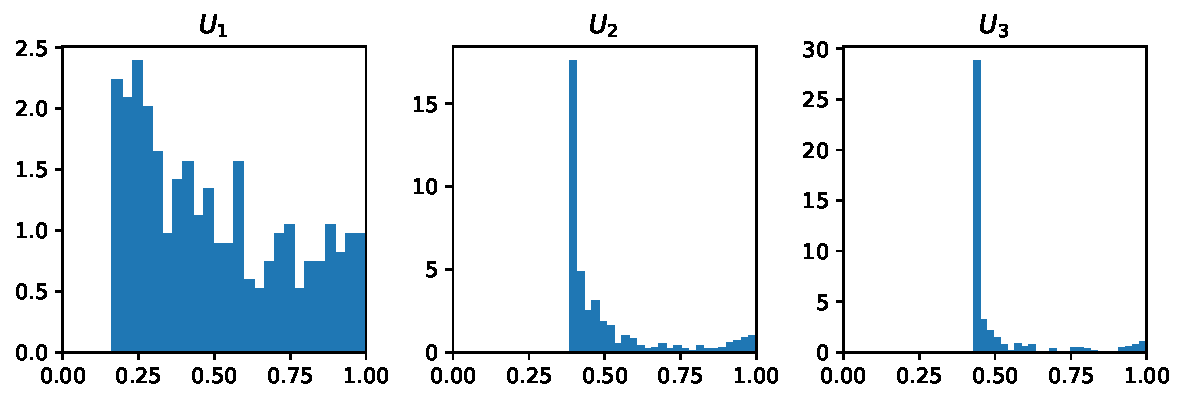
\includegraphics[width=0.99\linewidth]{figures/ND examples/Gaussian 3x3 large s uniforms.pdf}
        \caption{The samples transformed using $U_i = F_i(X_i)$ for $\boldsymbol\sigma = (1,2,3)$. These should be uniformly distributed, but clearly this is not the case for $U_2$ and $U_3$. Even $U_1$ does not quite resemble $10{,}000$ samples from a uniform distribution.}
        \label{fig:Gaussian 3x3 large s uniforms}
    \end{figure}
    \begin{table}[h]
        \centering
        \begin{tabular}{c|c|c|c}
                    & $U_1$    & $U_2$   & $U_3$   \\\hline
            $D_n$   & 0.066209 & 0.36014 & 0.46285 \\
            p-value & 0        & 0       & 0
        \end{tabular}
        \caption{based on 10,000 samples for $\boldsymbol\sigma = (1, 2, 3)$.}
    \end{table}
    Before handling this, the non-uniformity of $U_1$ in \autoref{fig:Gaussian 3x3 large s uniforms} is likely also present in the case when $\boldsymbol\sigma = (1,1,1)$. Indeed, \autoref{fig:Gaussian 3x3 medium s uniforms} shows that this is indeed the case.
    \begin{figure}[H]
        \centering
        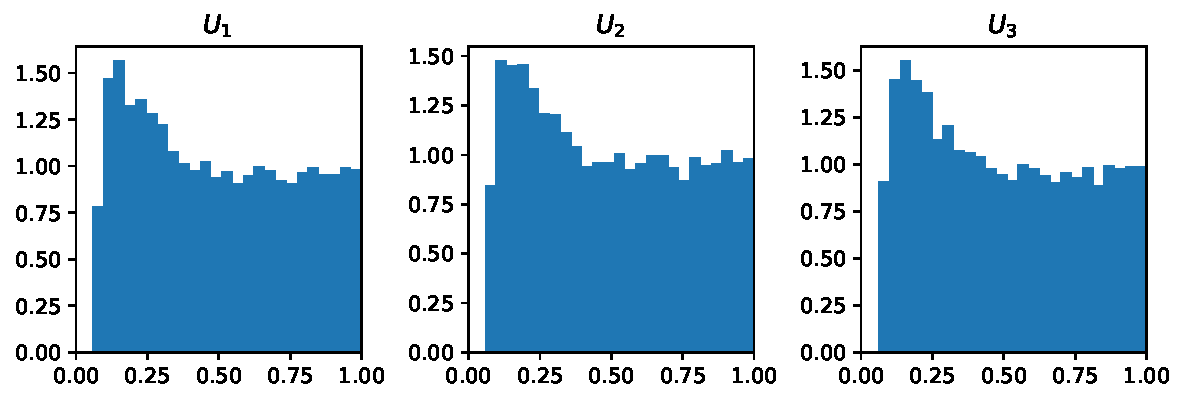
\includegraphics[width=0.99\linewidth]{figures/ND examples/Gaussian 3x3 medium s uniforms.pdf}
        \caption{The samples transformed using $U_i = F_i(X_i)$ for $\boldsymbol\sigma = (1,1,1)$.}
        \label{fig:Gaussian 3x3 medium s uniforms}
    \end{figure}
    \begin{table}[h]
        \centering
        \begin{tabular}{c|c|c|c}
                    & $U_1$    & $U_2$    & $U_3$    \\\hline
            $D_n$   & 0.068408 & 0.066808 & 0.070809 \\
            p-value & 0        & 0        & 0
        \end{tabular}
        \caption{based on 10,000 samples for $\boldsymbol\sigma = (1, 1, 1)$.}
    \end{table}
    Finally, just to be sure, $\boldsymbol\sigma = (0.07, 0.3, 0.9)$ is also shown in \autoref{fig:Gaussian 3x3 small s uniforms} and seems very reasonable, except for $U_3$.
    \begin{figure}[H]
        \centering
        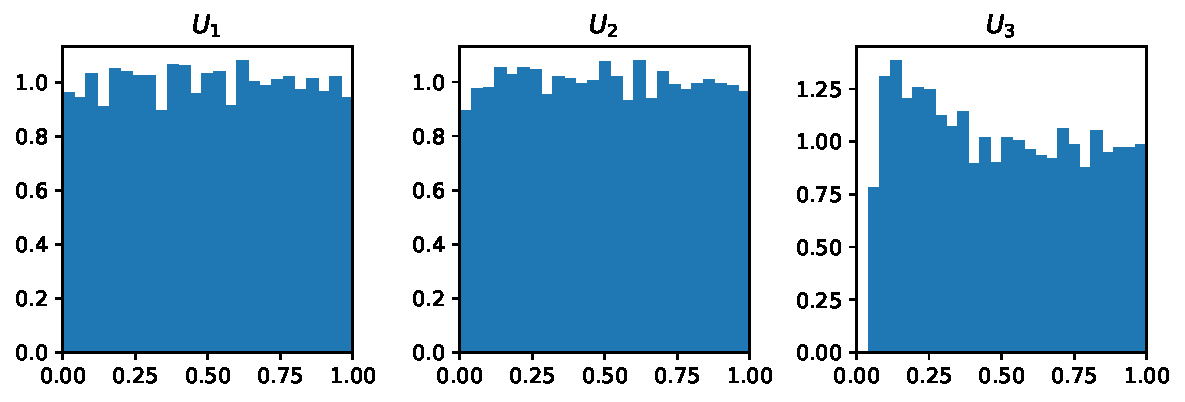
\includegraphics[width=0.99\linewidth]{figures/ND examples/Gaussian 3x3 small s uniforms.pdf}
        \caption{\raggedright The samples transformed using $U_i = F_i(X_i)$ for $\boldsymbol\sigma = (0.07, 0.3, 0.9)$.\hfill}
        \label{fig:Gaussian 3x3 small s uniforms}
    \end{figure}
    \begin{table}[h]
        \centering
        \begin{tabular}{c|c|c|c}
                    & $U_1$      & $U_2$     & $U_3$    \\\hline
            $D_n$   & 0.00581897 & 0.0068066 & 0.050908 \\
            p-value & 0.88645    & 0.74179   & 0
        \end{tabular}
        \caption{based on 10,000 samples for $\boldsymbol\sigma = (0.07, 0.3, 0.9)$.}
    \end{table}
    From the above examples, it seems that the larger the variance, the worse the uniforms turn out. Reasons for this could include numerical issues when trying to calculate $u_i^{(j)}$ form $y_i^{(j)}$ by $u_i^{(j)} = \int_{-\infty}^{y_i^{(j)}} f_i(y) \, dy$ and bad fitting of the kernel density estimate from observations. In particular, for values similar, which happens in the case for large $\sigma$ such that we observe large negative realizations of $X_i$, $y_i^{(j)}$ are almost 0, and when computing the integral could result in identical values. Furthermore, from \autoref{fig:Gaussian 3x3 large s X3 KDE} we see that indeed the fit is quite poor. Note that we have zoomed in on the interval $[-200 , 200]$ which contains $96.2\%$ of observations. The poor fit is primarily due to the use of Scott's Rule \textcolor{red}{as discussed above} which in this case overshoots the optimal bandwidth by a lot.
    \begin{figure}[H]
        \centering
        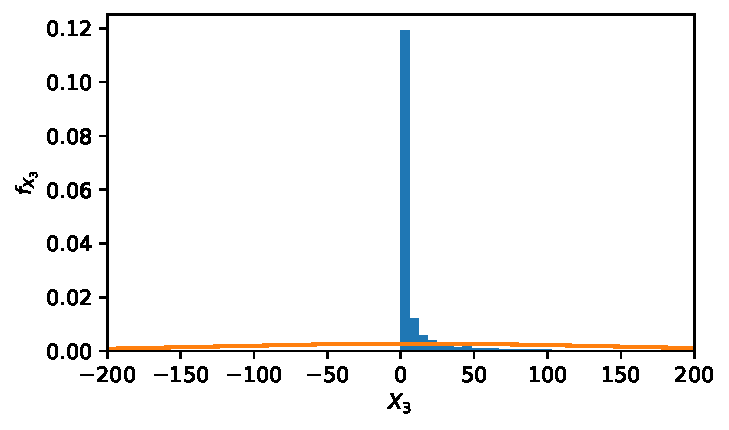
\includegraphics[width=0.7\linewidth]{figures/ND examples/Gaussian 3x3 large s X3 KDE.pdf}
        \caption{}
        \label{fig:Gaussian 3x3 large s X3 KDE}
    \end{figure}
    The poor fit also explains the high concentration of $U_3$ around $0.5$ in \autoref{fig:Gaussian 3x3 large s uniforms} as only $54.5\%$ of the probability mass lies above $0$.

    However, also here \autoref{coro: Coordinate transformation} proves to be useful. Namely, we can get rid of the numerical issues by transforming $Y_i$ using e.g. $\log(\cdot)$ or $(\cdot)^{p}$ for $p>0$ to get even out the observations more. As the first simply inverts the initial transformation of $X_i$, we choose the latter as a more interesting case. In particular, choosing $p<1$ will result in a more even distribution. In the following, $p=1/10$ has been used to transform $\boldsymbol Y$ prior to running \autoref{alg:Gobs1} and the resulting $u_i^{(j)}$ is shown in \autoref{fig:Gaussian 3x3 large s power uniforms}.
    \begin{figure}[H]
        \centering
        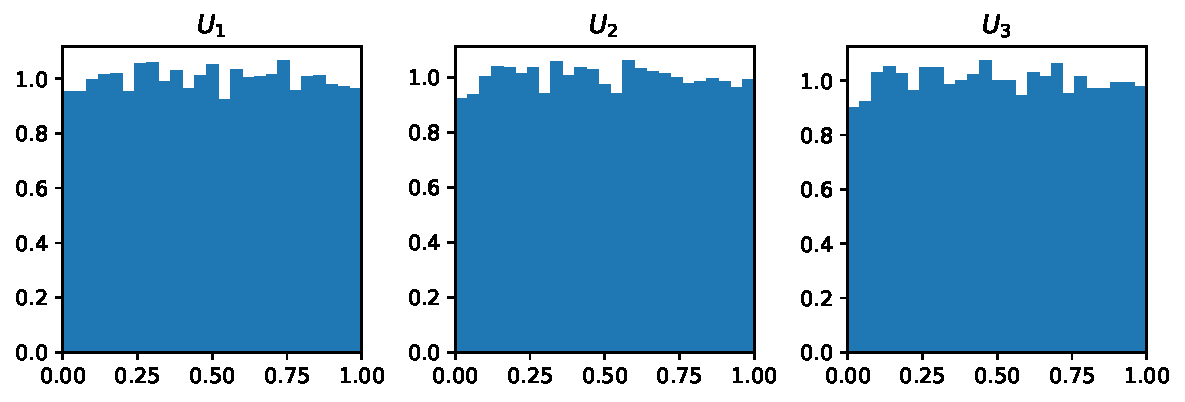
\includegraphics[width=0.99\linewidth]{figures/ND examples/Gaussian 3x3 large s power uniforms.pdf}
        \caption{}
        \label{fig:Gaussian 3x3 large s power uniforms}
    \end{figure}
    \begin{table}[h]
        \centering
        \begin{tabular}{c|c|c|c}
                    & $U_1$     & $U_2$     & $U_3$     \\\hline
            $D_n$   & 0.0061099 & 0.0061435 & 0.0073148 \\
            p-value & 0.84838   & 0.84368   & 0.65690
        \end{tabular}
        \caption{based on 10,000 samples for $\boldsymbol\sigma = (1, 2, 3)$ with power transform.}
    \end{table}
    The resulting $u_i^{(j)}$ now seem to follow a uniform distribution and indeed the KDE fits much better as seen in \autoref{fig:Gaussian 3x3 large s power X3 KDE}.
    \begin{figure}[H]
        \centering
        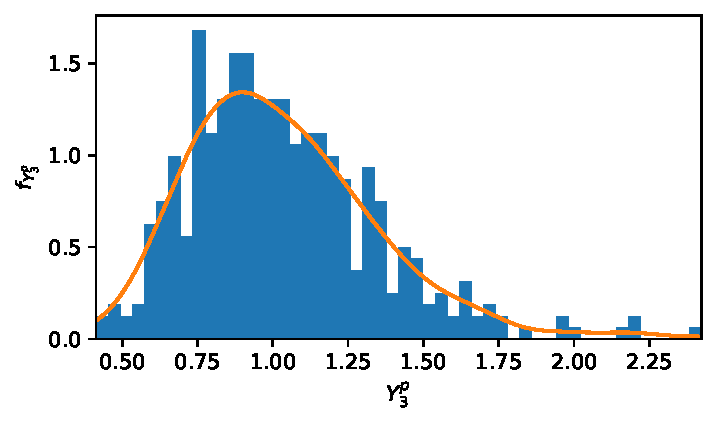
\includegraphics[width=0.7\linewidth]{figures/ND examples/Gaussian 3x3 large s power X3 KDE.pdf}
        \caption{}
        \label{fig:Gaussian 3x3 large s power X3 KDE}
    \end{figure}
    Turning to \autoref{alg:Gobs1} and \autoref{alg:ND} we now find that $G_{dir}$ is given by
    $$G_{dir} =
        \begin{bmatrix}
            -0.3290  & 0.6610   & 0.008440   \\
            0.6610   & -0.3290  & 0.008150   \\
            0.008440 & 0.008150 & -0.0002061
        \end{bmatrix}
    $$
    Which is indeed much more comparable with the result from before in \autoref{eq:s medium G_dir} and \autoref{eq:s small G_dir}. The difference between $G_{dir}$ from $\boldsymbol Y$ and $\boldsymbol Y^p$ is clearly visible in \autoref{fig:Gaussian 3x3 large s G_dir differences} and also \autoref{fig:Gaussian 3x3 large s power} resembles the original correlation structure.
    \begin{figure}[H]
        \centering
        \begin{subfigure}[t]{0.49\textwidth}
            \centering
            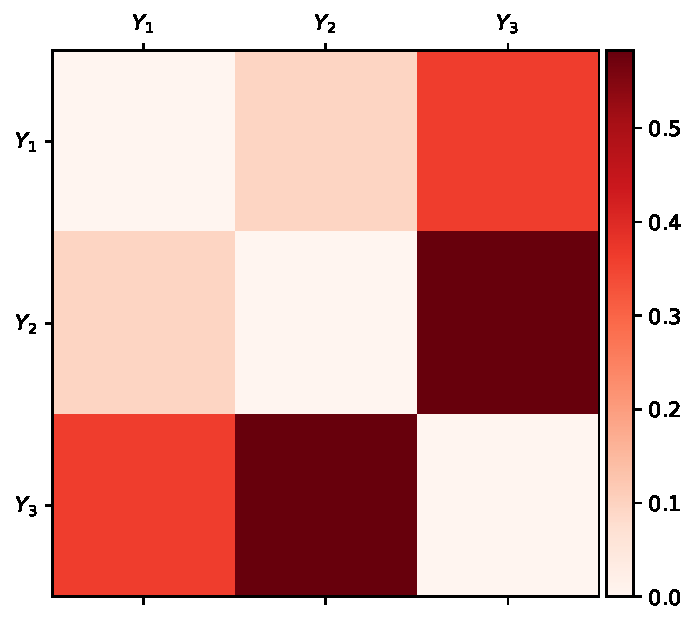
\includegraphics[width=\linewidth]{figures/ND examples/Gaussian 3x3 large s.pdf}
            \caption{}
            \label{fig:Gaussian 3x3 large s}
        \end{subfigure}%
        ~
        \begin{subfigure}[t]{0.49\textwidth}
            \centering
            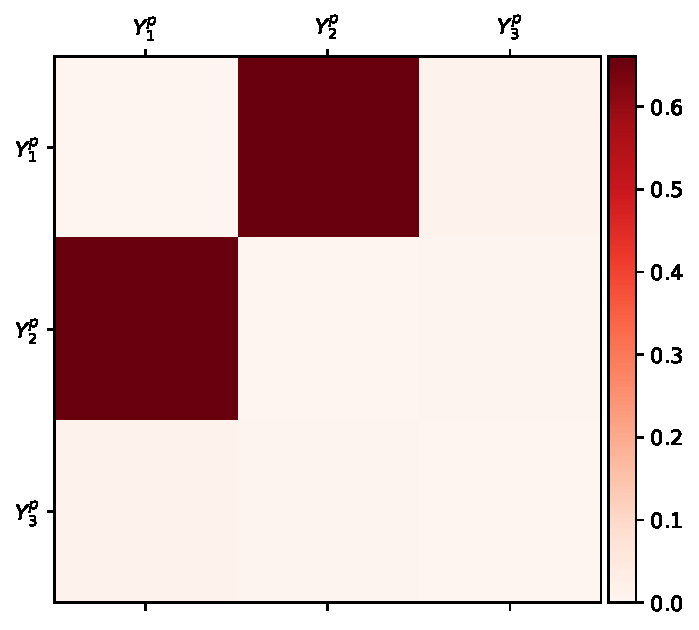
\includegraphics[width=\linewidth]{figures/ND examples/Gaussian 3x3 large s power.pdf}
            \caption{}
            \label{fig:Gaussian 3x3 large s power}
        \end{subfigure}
        \caption{$G_{dir}$ resulting from $10{,}000$ samples from multi variate Gaussian with $\boldsymbol\sigma = (1,2,3)$ in \textbf{(a)} with raw samples from $\boldsymbol Y$ and in \textbf{(b)} the transformed data corresponding to $\boldsymbol Y^p$.}
        \label{fig:Gaussian 3x3 large s G_dir differences}
    \end{figure}
    Finally, to end this example we shall compare with some theoretical results. Namely, the output $G_{obs}$ of \autoref{alg:Gobs1} can also be calculated theoretically. For this, we shall use \autoref{prop:MI bivariate gaussian} which permits a theoretical result, namely
    \begin{align*}
        G_{obs} & =
        \begin{bmatrix}
            0                                              & -\frac{1}{2} \ln \left( 1 - \rho_{12}^2\right) & -\frac{1}{2} \ln \left( 1 - \rho_{13}^2\right) \\
            -\frac{1}{2} \ln \left( 1 - \rho_{21}^2\right) & 0                                              & -\frac{1}{2} \ln \left( 1 - \rho_{23}^2\right) \\
            -\frac{1}{2} \ln \left( 1 - \rho_{31}^2\right) & -\frac{1}{2} \ln \left( 1 - \rho_{32}^2\right) & 0
        \end{bmatrix} \\
                & \cong
        \begin{bmatrix}
            0       & 0.83037 & 0 \\
            0.83037 & 0       & 0 \\
            0       & 0       & 0
        \end{bmatrix}
    \end{align*}
    Similarly, prior to deconvolution, using just the sampled $\boldsymbol X$ (i.e. no exponential transform), \autoref{alg:Gobs1} returns
    $$G_{obs} =
        \begin{bmatrix}
            0.         & 0.71841756 & 0.01781815 \\
            0.71841756 & 0.         & 0.01769672 \\
            0.01781815 & 0.01769672 & 0.
        \end{bmatrix}
    $$
    \textcolor{red}{Test om denne G er lige den teoretiske. Eller nærmere, argumenter for hvorfor vi ikke laver en test, eller hvad man kunne gøre. Har samplet fra en simultan normalfordeling, så kan lave en til en mellem MI og korrelation. }

    From the confidence density for the correlation $\rho$ given the emperical correlation $r$ is given by
    $$f\left(\rho \mid r,\nu\right) = \frac{\nu (\nu-1) \Gamma(\nu-1)}{\sqrt{2\pi} \Gamma(\nu + \frac{1}{2})} \frac{\left(1-r^2\right)^{\frac{\nu-1}{2}} \left(1-\rho^2\right)^{\frac{\nu-2}{2}} }{\left(1-r\rho\right)^{\frac{2\nu-1}{2}}} F\left(\frac{3}{2}, -\frac{1}{2}, \nu+\frac{1}{2}, \frac{1+r\rho}{2}\right)$$
    from the mutual information, we can calculate the absolute correlation. Notice that the density does not change when reversing both $r$ and $\rho$ simultaneously, thus, without loss of generality, assume $r\geq 0$, then we can calculate a CI for $\rho$ (which will be negated if we had used $-r$ instead and thus would be identical when taking the absolute value). If the original CI $[a,b]$ contains $0$ i.e. $a<0$, we shall write the CI for the absolute correlation as $[0,b]$ instead. This way, we can compare the absolute correlations and see if they are the same (by checking if the CI contains the theoretical correlation) by \cite{Confidence-in-Correlation}. Using numerical integration (fast enough with high numerical accuracy from many bins, 1 mil bins, yielding probability mass 1.0000000000008133), can compute CI for absolute correlation

    \autoref{sec:bivar gauss abs correlation CI}


    Clearly these are not equal, but in this case, the error is suspected to originate from the estimated joint density. For example, considering $X_1$ and $X_2$, we compare the estimated joint copula density and compare to the theoretical \textcolor{red}{reference til et sted hvor gausisk copula står} shown in \autoref{fig:gaussian copula estimate} and \autoref{fig:gaussian copula truth} respectively.
    \begin{figure}[H]
        \centering
        \begin{subfigure}[t]{0.45\linewidth}
            \centering
            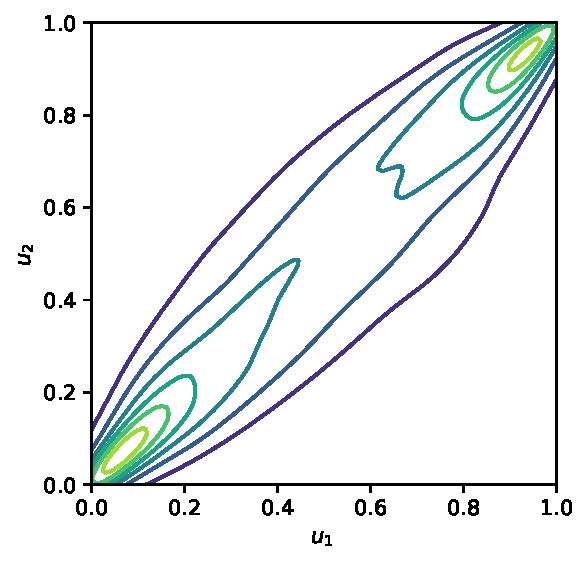
\includegraphics[width = \linewidth]{figures/ND examples/Gaussian copula sample contour.pdf}
            \caption{}
        \end{subfigure}%
        ~
        \begin{subfigure}[t]{0.5\linewidth}
            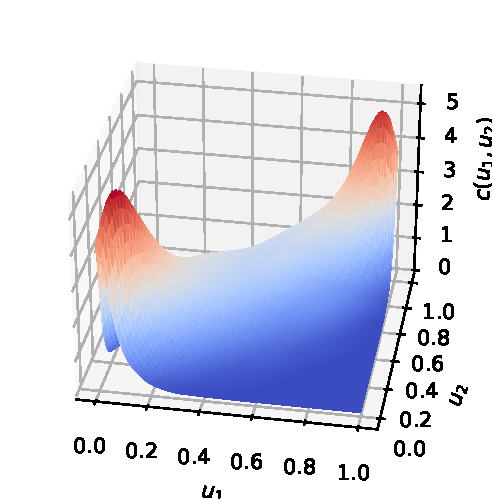
\includegraphics[width = \linewidth]{figures/ND examples/Gaussian copula sample pdf.pdf}
            \caption{}
        \end{subfigure}
        \caption{Estimated copula density $c$ with $\rho = 0.9$ corresponding to $X_1$ and $X_2$.}
        \label{fig:gaussian copula estimate}
    \end{figure}
    The noticeable difference is in the corners $(0,0)$ and $(1,1)$ where the theoretical copula density tends to infinity whereas the estimated density has modes at $(0.1,0.1)$ and $(0.9,0.9)$. In particular, simply rescaling the copula density in \autoref{alg:Gobs1} does not resemble the theoretical boundary which is a known issue \textcolor{red}{reference til artikel om undershoot peaks og boundary conditions for KDE}. A better approach may be to use jackknifing \textcolor{red}{link til afsnit of jackknifing, som også indeholder reference til artikel hvor dette gøres}.
    \begin{figure}[H]
        \centering
        \begin{subfigure}[t]{0.45\linewidth}
            \centering
            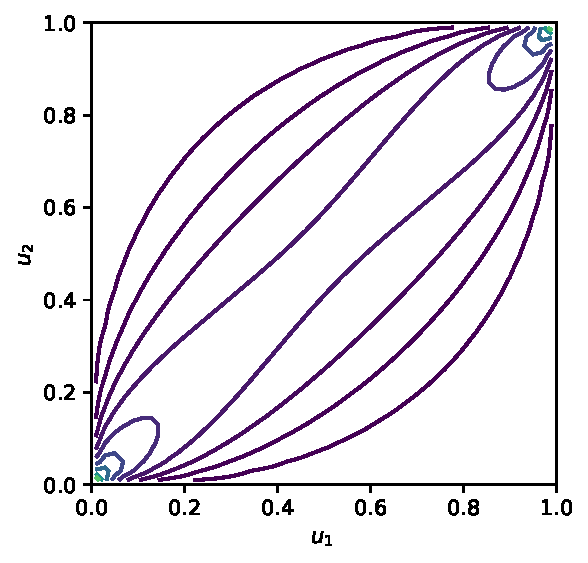
\includegraphics[width = \linewidth]{figures/ND examples/Gaussian copula theoretical contour.pdf}
            \caption{}
        \end{subfigure}%
        ~
        \begin{subfigure}[t]{0.5\linewidth}
            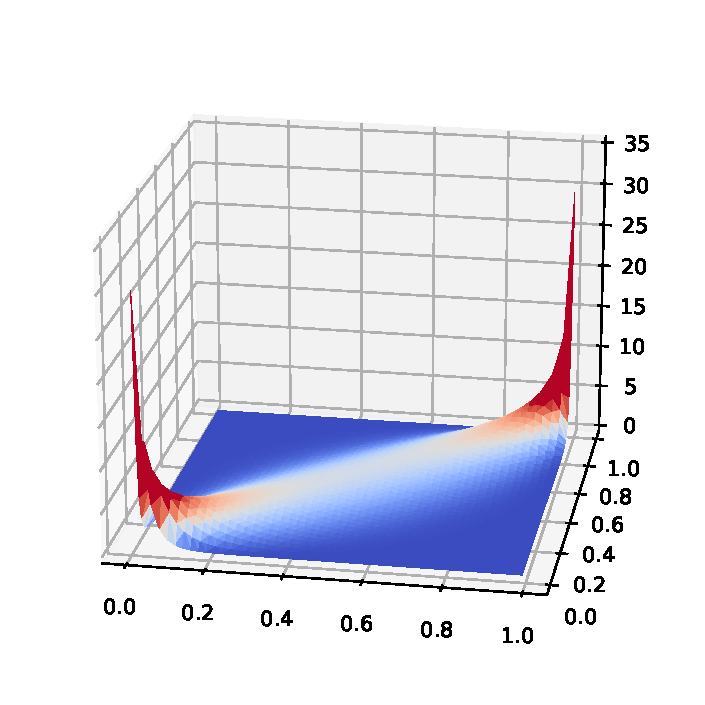
\includegraphics[width = \linewidth]{figures/ND examples/Gaussian copula theoretical pdf.pdf}
            \caption{}
        \end{subfigure}
        \caption{Theoretical copula density $c$ with $\rho = 0.9$ corresponding to $X_1$ and $X_2$.}
        \label{fig:gaussian copula truth}
    \end{figure}
    We note however, that the underlying structure is still captured i.e. that $Y_1$ and $Y_2$ covary while $Y_3$ does not inform $Y_1$ or $Y_2$ and vice versa.
\end{example}

We continue with a similar example to the previous one. The key difference is the number of variables and a more complicated correlation structure to test the algorithms further.
\begin{example}
    From \autoref{ex:1} we saw how one could handle some numerical issues. Thus, in this example we shall not bother ourselves with such computations and merely focus on the correlation structure. In particular, we shall sample $\boldsymbol X$ from a 10 dimensional
\end{example}


\newpage

\section{sammenligning af metoder for at finde MI}
Sammenligning af gammel metode og "min"
\begin{figure}[h]
    \centering
    \begin{subfigure}[t]{0.49\textwidth}
        \centering
        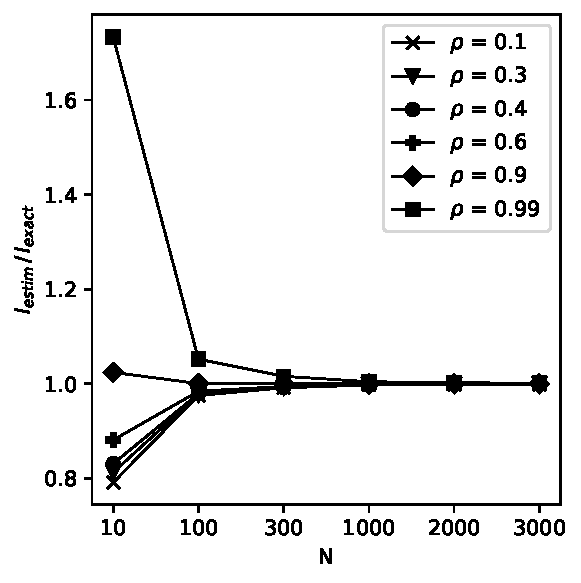
\includegraphics[width=\linewidth]{figures/ND examples/MI calc/gaussian example all.pdf}
        \caption{}
        \label{subfig:new MI method all}
    \end{subfigure}%
    ~
    \begin{subfigure}[t]{0.49\textwidth}
        \centering
        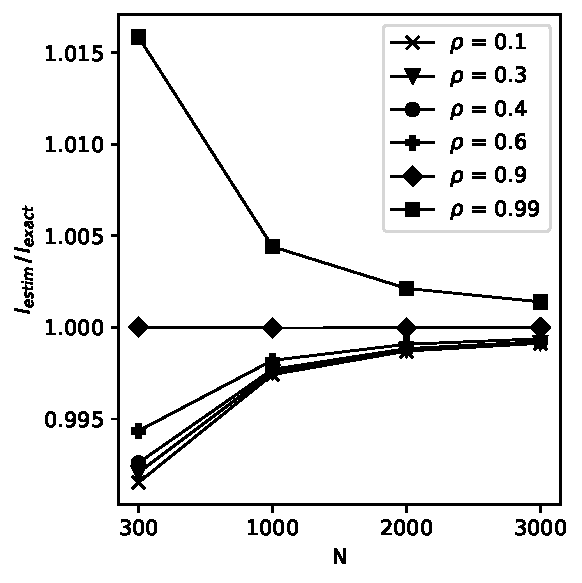
\includegraphics[width=\linewidth]{figures/ND examples/MI calc/gaussian example zoom.pdf}
        \caption{}
        \label{subfig:new MI method all zoom}
    \end{subfigure}
    \caption{Evaluation of MI for new method for different N. \textcolor{red}{Bør sammenlignes med artiekl fundet (har sat i bibtex) og original papers (ikke Kina)}}
    \label{fig:dd}
\end{figure}

\begin{figure}[h]
    \centering
    \begin{subfigure}[t]{0.32\textwidth}
        \centering
        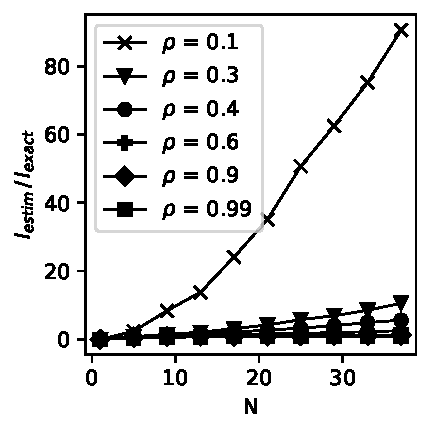
\includegraphics[width=\linewidth]{figures/ND examples/MI calc/gaussian example original all.pdf}
        \caption{}
        \label{subfig:d}
    \end{subfigure}%
    ~
    \begin{subfigure}[t]{0.32\textwidth}
        \centering
        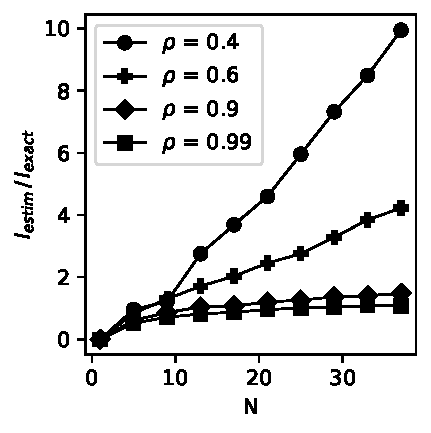
\includegraphics[width=\linewidth]{figures/ND examples/MI calc/gaussian example original zoom.pdf}
        \caption{}
        \label{subfig:dd}
    \end{subfigure}%
    ~
    \begin{subfigure}[t]{0.32\textwidth}
        \centering
        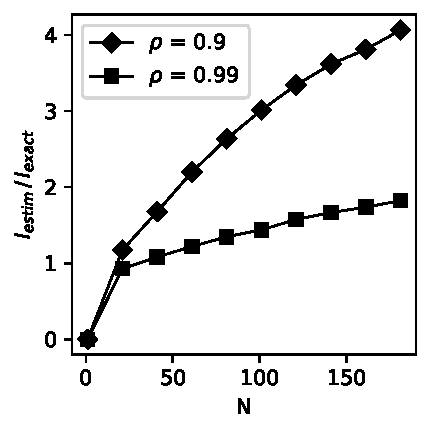
\includegraphics[width=\linewidth]{figures/ND examples/MI calc/gaussian example original high corr.pdf}
        \caption{}
        \label{subfig:ddd}
    \end{subfigure}
    \caption{Evaluation of MI for old method for different N. Ligner der er knæk ved fporhold lig 1. Men ved næremere undersøgelse blev det fundet ud af at det ikke helt er tilfældet, og derudover vil der skulle laves en algoritmisk måde at finde dette knæk på. Savitzky–Golay filter kunne være en mulighed, eller gruppere e.g. 5 forskellige bins og tag gennemsnit. Efter smoothing kan anden afledte tæt på 0 bruges, til at finde hvornår stykket bliver fladt (tilnærmelses vist)}
    \label{fig:ddd}
\end{figure}

\textcolor{red}{ved høj korrelation i.e. tæt på laver dimensionel manifold, skal der bruges mange, som i rigtig mange samples i mesh. }


\textcolor{red}{Inkluder flere exempler end blot gaussian as done by \cite{Estimating-mutual-information-Kraskov}}

\subsection{10D gaussian example}
\textcolor{red}{casuality svarer til at lave nedre/øvre trekant. Er der forskel i at gør edet før og efter for en symmetrisk matrix? - Ja, men begge metoder på 10 eksempel giver gode resultater. Kommenter at det er matematisk meget forskelligt at filtrere først og så ND efter og omvendt}



\end{document}